\documentclass{article}
\usepackage{amsmath}
\usepackage{amssymb}
\usepackage{amsthm}
\usepackage{graphicx}

\title{Préambule du projet capteur actionneur}
\author{AVRIL Théo, LERISSEL Elouen}
\date{\today}

\begin{document}
    \maketitle
    Test
    \tableofcontents
    \section{Introduction}
    \subsection{Contexte}
    \subsection{Objectif}
    \subsection{Méthodologie}
    \section{Séance 1}

    \subsection*{Calcul du prédiviseur et de la période du compteur}

    Nous souhaitons configurer un timer selon la formule suivante :
    
    \[
    P = \frac{(1 + \text{counter\_period}) \times (1 + \text{prescaler})}{F}
    \]
    
    où :
    \begin{itemize}
        \item $P$ est la période désirée en secondes ;
        \item $\text{counter\_period}$ est la valeur maximale du compteur ;
        \item $\text{prescaler}$ est la valeur du prédiviseur ;
        \item $F$ est la fréquence d'horloge du timer.
    \end{itemize}
    
    Dans notre cas :
    \[
    P = 0{,}25~\text{s} \quad \text{et} \quad F = 84~\text{MHz} = 84 \times 10^6~\text{Hz}
    \]
    
    En remplaçant dans l’équation :
    
    \[
    0{,}25 = \frac{(1 + \text{counter\_period}) \times (1 + \text{prescaler})}{84 \times 10^6}
    \]
    
    \[
    (1 + \text{counter\_period}) \times (1 + \text{prescaler}) = 0{,}25 \times 84 \times 10^6 = 21~000~000
    \]
    
    Nous cherchons deux entiers tels que :
    \[
    (1 + \text{counter\_period}) \times (1 + \text{prescaler}) = 21~000~000
    \quad \text{avec} \quad \text{counter\_period} \leq 65535, \quad \text{prescaler} \leq 65535
    \]
    
    On choisit la plus grande valeur possible pour le compteur afin de minimiser le prédiviseur :
    
    \[
    1 + \text{counter\_period} = 65536 \Rightarrow \text{counter\_period} = 65535
    \]
    
    \[
    1 + \text{prescaler} = \frac{21~000~000}{65536} \approx 320.4 \Rightarrow \text{prescaler} = 319
    \]
    
    \paragraph{Vérification :}
    
    \[
    P = \frac{65536 \times 320}{84 \times 10^6} = \frac{20~971~520}{84~000~000} \approx 0{,}24966~\text{s} \approx 249{,}66~\text{ms}
    \]
    
    \paragraph{Configuration PWM :}
    
    Nous avons configuré le timer en mode PWM, canal 2. Le paramètre \texttt{Pulse} a été défini à \textbf{3}, ce qui correspond à une valeur sur 16 bits. Cette configuration permet de générer un signal PWM avec un temps d’activation très court par rapport à la période complète.
    
    \paragraph{Conclusion :}
    
    Pour obtenir une période de $250~\text{ms}$ avec une fréquence d’horloge de $84~\text{MHz}$, la configuration suivante a été retenue :
    \begin{itemize}
        \item \textbf{counter\_period = 65535}
        \item \textbf{prescaler = 319}
        \item \textbf{PWM Generation Channel 2, Pulse = 3 (valeur 16 bits)}
    \end{itemize}

    \begin{figure}[htbp]
        \centering
        \begin{minipage}{0.45\textwidth}
            \centering
            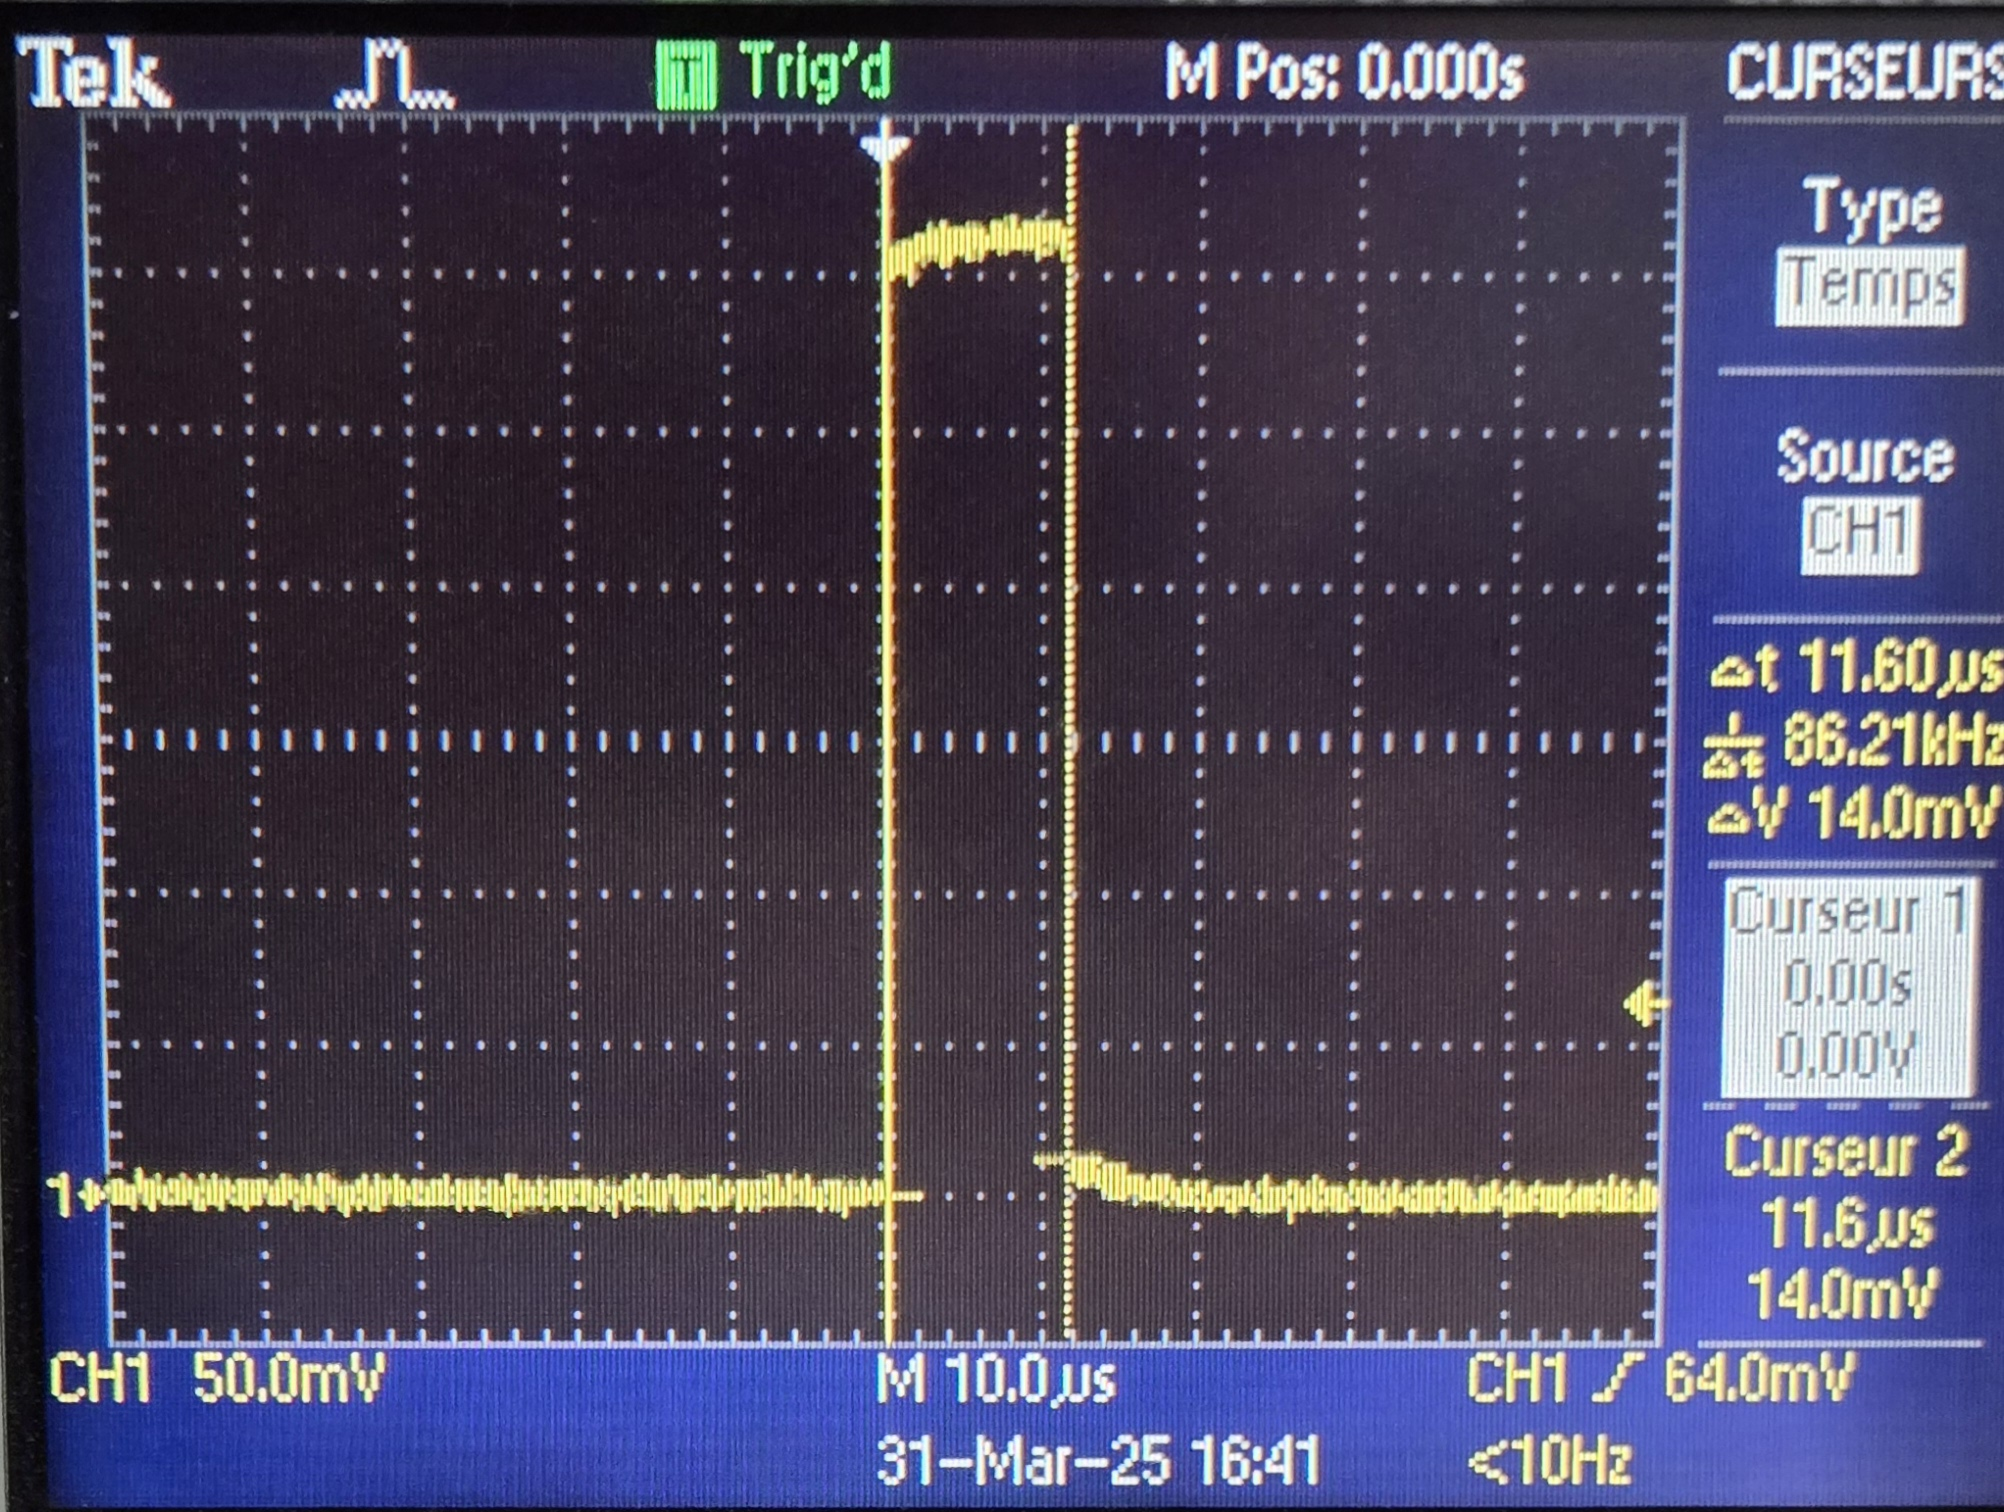
\includegraphics[width=\textwidth]{img/input_sr-04.jpg}
            \caption{Signal d'entrée du capteur HC-SR04}
            \label{fig:input_sr-04}
        \end{minipage}
        \hfill
        \begin{minipage}{0.45\textwidth}
            \centering
            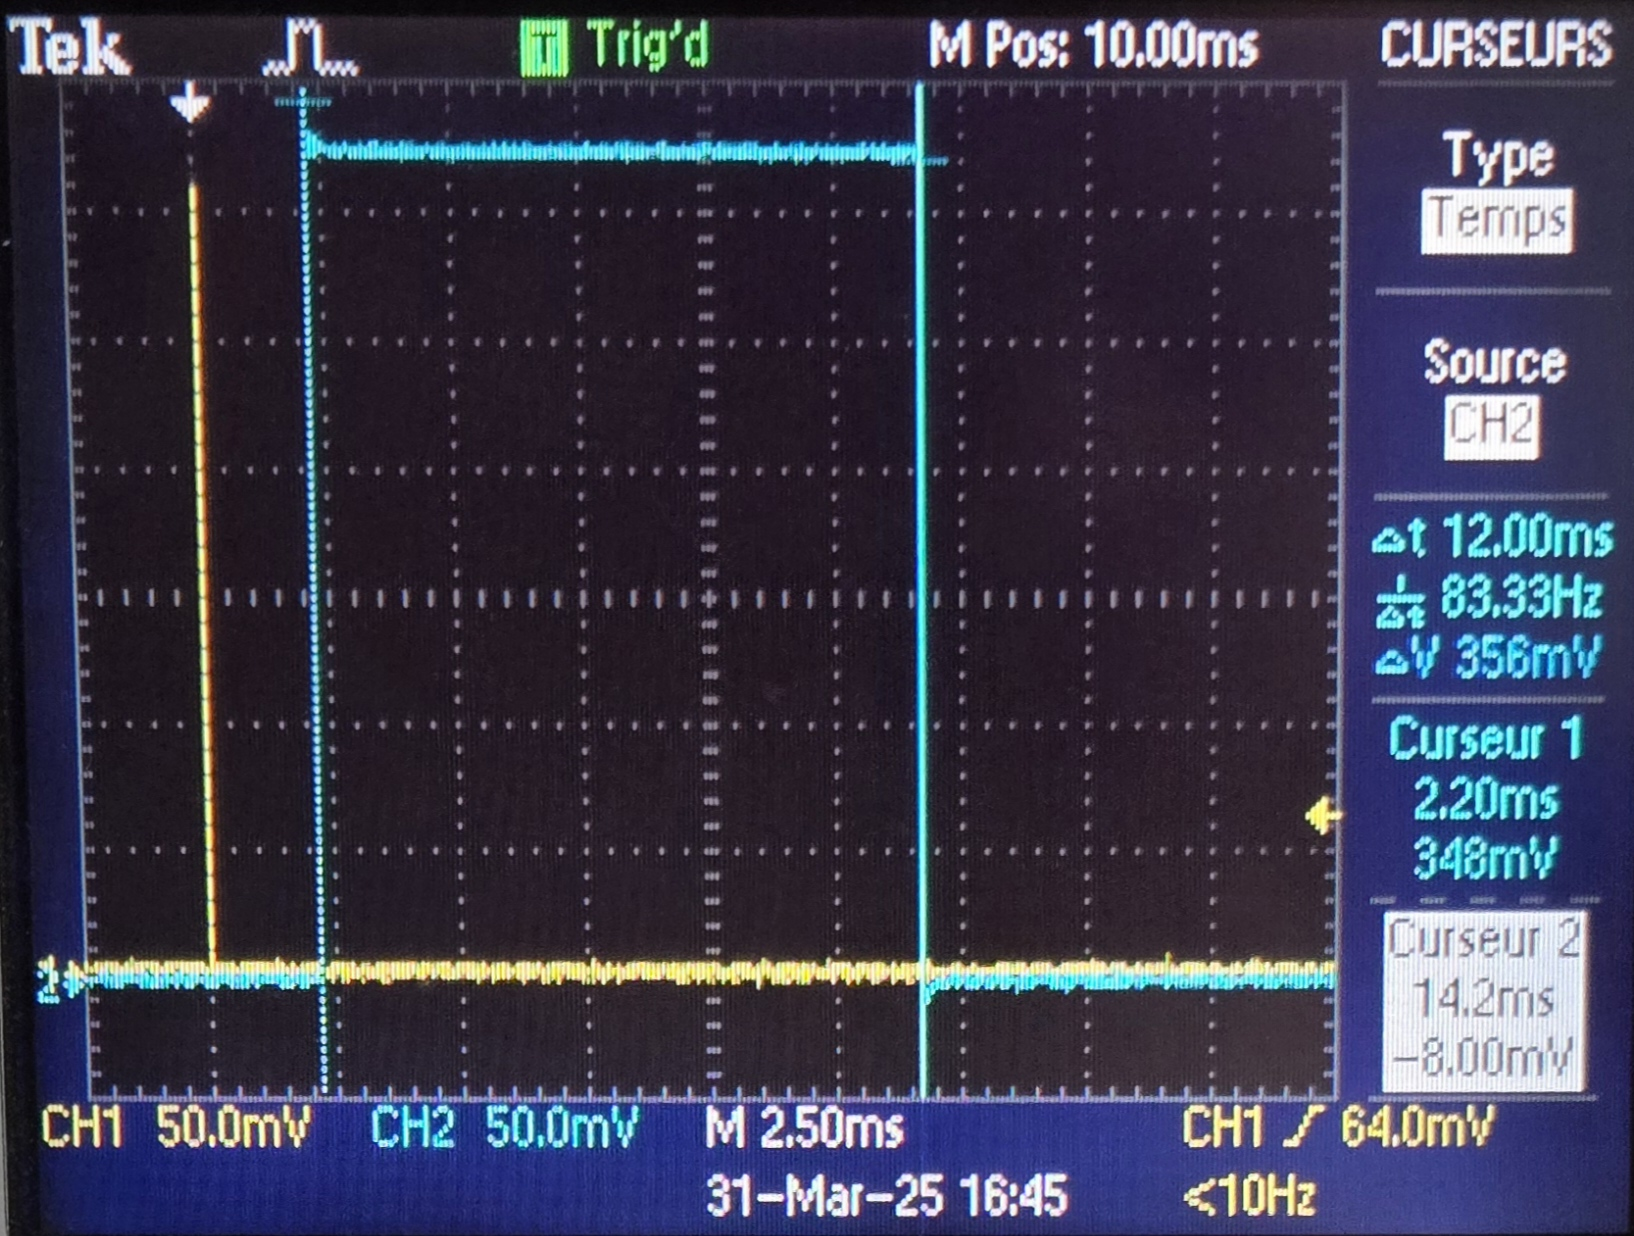
\includegraphics[width=\textwidth]{img/output_sr-04.jpg}
            \caption{Signal de sortie du capteur HC-SR04}
            \label{fig:output_sr-04}
        \end{minipage}
    \end{figure}

    \subsection*{Gestion des interruptions EXTI}

Dans le cadre de notre projet, nous avons utilisé le capteur à ultrasons HC-SR04 pour mesurer des distances. Ce capteur envoie un signal haut (ECHO) lorsque l’onde ultrasonore émise est réfléchie par un obstacle et revient au capteur. Pour mesurer avec précision le temps entre l’émission et la réception de l’onde, il est essentiel de détecter le front montant du signal ECHO, qui marque le début de ce temps de vol.

Pour cela, nous avons utilisé les interruptions EXTI (External Interrupt) disponibles sur le microcontrôleur STM32. Le principe est simple : configurer une broche GPIO en entrée, et la relier à une ligne d'interruption externe déclenchée sur un front montant ou descendant.

Dans STM32CubeMX, nous avons commencé par configurer la broche connectée au signal ECHO du capteur en mode \textbf{GPIO Input}, avec l'option \textbf{External Interrupt Mode with Rising/Falling Edge Trigger}. Cela signifie que dès que le signal ECHO passe de l'état bas à l'état haut, une interruption est générée automatiquement.

Nous avons ensuite activé cette interruption dans l’onglet NVIC (Nested Vectored Interrupt Controller) de CubeMX, afin que le microcontrôleur prenne bien en compte l’événement et déclenche le traitement associé.

Une fois le code généré, nous avons implémenté la fonction de rappel \texttt{HAL\_GPIO\_EXTI\_Callback()}, fournie par la HAL (Hardware Abstraction Layer) de ST. Cette fonction est appelée automatiquement à chaque interruption externe. À l'intérieur, nous avons vérifié que la broche concernée était bien celle du capteur HC-SR04, et si c’est le cas, nous avons exécuté le traitement désiré, à savoir le début du chronométrage pour mesurer la durée du signal ECHO.

Voici un exemple simplifié du code utilisé :

\begin{verbatim}
void HAL_GPIO_EXTI_Callback(uint16_t GPIO_Pin)
{
    if (GPIO_Pin == GPIO_PIN_X) // Remplacer GPIO_PIN_X par la broche utilisée
    {
        // Début de la mesure du temps de vol
    }
}
\end{verbatim}

Cette méthode nous permet de réagir immédiatement à l’arrivée du front montant, sans avoir besoin de scruter la broche en permanence dans la boucle principale (polling). Elle est donc bien plus efficace et adaptée à notre besoin de précision temporelle dans le cadre de la mesure de distance.



\end{document}